\documentclass{standalone}
\usepackage{tikz}
\usetikzlibrary{patterns, positioning}


\begin{document}
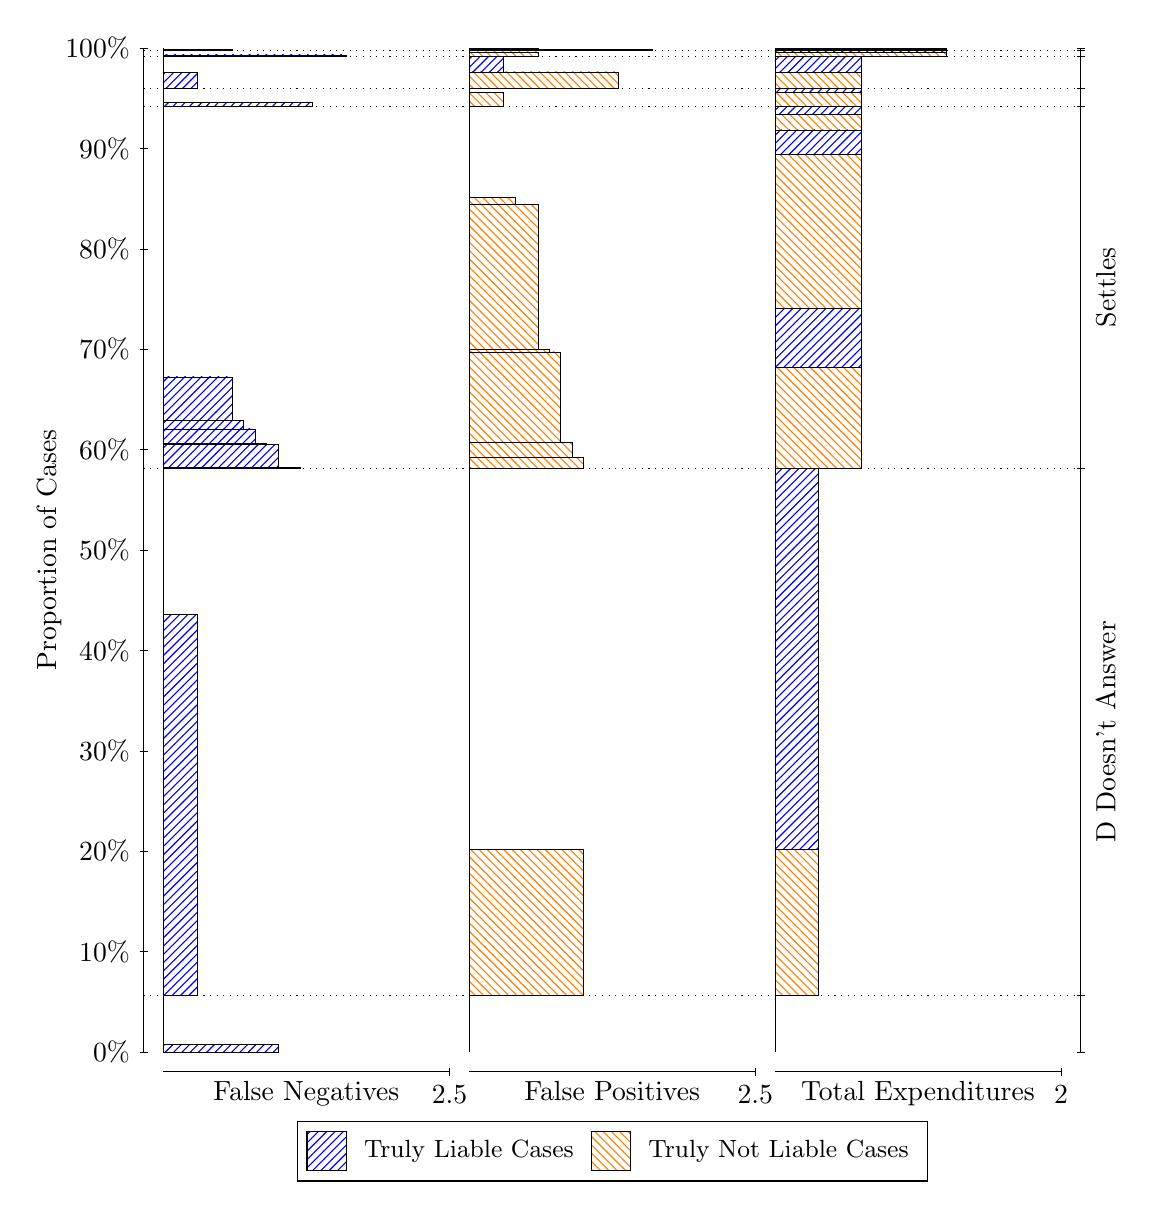
\begin{tikzpicture}
\draw[black, very thin] (1.5,1.75) -- (1.5,14.5);
\node[rotate=90, text=black, anchor=center] at (0.3, 8.125) {Proportion of Cases};
\draw[black, very thin] (1.45,1.75) -- (1.55,1.75);
\node[text=black, anchor=east] at (1.45, 1.75) {0\%};
\draw[black, very thin] (1.45,3.025) -- (1.55,3.025);
\node[text=black, anchor=east] at (1.45, 3.025) {10\%};
\draw[black, very thin] (1.45,4.3) -- (1.55,4.3);
\node[text=black, anchor=east] at (1.45, 4.3) {20\%};
\draw[black, very thin] (1.45,5.575) -- (1.55,5.575);
\node[text=black, anchor=east] at (1.45, 5.575) {30\%};
\draw[black, very thin] (1.45,6.85) -- (1.55,6.85);
\node[text=black, anchor=east] at (1.45, 6.85) {40\%};
\draw[black, very thin] (1.45,8.125) -- (1.55,8.125);
\node[text=black, anchor=east] at (1.45, 8.125) {50\%};
\draw[black, very thin] (1.45,9.4) -- (1.55,9.4);
\node[text=black, anchor=east] at (1.45, 9.4) {60\%};
\draw[black, very thin] (1.45,10.675) -- (1.55,10.675);
\node[text=black, anchor=east] at (1.45, 10.675) {70\%};
\draw[black, very thin] (1.45,11.95) -- (1.55,11.95);
\node[text=black, anchor=east] at (1.45, 11.95) {80\%};
\draw[black, very thin] (1.45,13.225) -- (1.55,13.225);
\node[text=black, anchor=east] at (1.45, 13.225) {90\%};
\draw[black, very thin] (1.45,14.5) -- (1.55,14.5);
\node[text=black, anchor=east] at (1.45, 14.5) {100\%};

\draw[black, very thin] (13.4,1.75) -- (13.4,14.5);
\draw[black, very thin] (13.35,1.75) -- (13.45,1.75);
\node[anchor=west] at (13.35, 1.75) {};
\draw[black, very thin] (13.35,2.4675) -- (13.45,2.4675);
\node[anchor=west] at (13.35, 2.4675) {};
\draw[black, very thin] (13.35,9.164) -- (13.45,9.164);
\node[anchor=west] at (13.35, 9.164) {};
\draw[black, very thin] (13.35,13.762) -- (13.45,13.762);
\node[anchor=west] at (13.35, 13.762) {};
\draw[black, very thin] (13.35,13.985) -- (13.45,13.985);
\node[anchor=west] at (13.35, 13.985) {};
\draw[black, very thin] (13.35,14.396) -- (13.45,14.396);
\node[anchor=west] at (13.35, 14.396) {};
\draw[black, very thin] (13.35,14.466) -- (13.45,14.466);
\node[anchor=west] at (13.35, 14.466) {};
\draw[black, very thin] (13.35,14.5) -- (13.45,14.5);
\node[anchor=west] at (13.35, 14.5) {};

\draw[black, very thin, pattern color=blue, pattern=north east lines] (1.75,1.75) rectangle (3.2033,1.8455);
\draw[black, very thin, pattern color=orange, pattern=north west lines] (1.75,1.8455) rectangle (1.75,2.4675);
\draw[black, very thin, pattern color=blue, pattern=north east lines] (1.75,2.4675) rectangle (2.186,7.3067);
\draw[black, very thin, pattern color=orange, pattern=north west lines] (1.75,7.3067) rectangle (1.75,9.164);
\draw[black, very thin, pattern color=blue, pattern=north east lines] (1.75,9.164) rectangle (3.494,9.1787);
\draw[black, very thin, pattern color=blue, pattern=north east lines] (1.75,9.1787) rectangle (3.2033,9.4643);
\draw[black, very thin, pattern color=blue, pattern=north east lines] (1.75,9.4643) rectangle (3.058,9.4743);
\draw[black, very thin, pattern color=blue, pattern=north east lines] (1.75,9.4743) rectangle (2.9127,9.6631);
\draw[black, very thin, pattern color=blue, pattern=north east lines] (1.75,9.6631) rectangle (2.7673,9.7683);
\draw[black, very thin, pattern color=blue, pattern=north east lines] (1.75,9.7683) rectangle (2.622,10.324);
\draw[black, very thin, pattern color=orange, pattern=north west lines] (1.75,10.324) rectangle (1.75,13.762);
\draw[black, very thin, pattern color=blue, pattern=north east lines] (1.75,13.762) rectangle (3.6393,13.807);
\draw[black, very thin, pattern color=orange, pattern=north west lines] (1.75,13.807) rectangle (1.75,13.985);
\draw[black, very thin, pattern color=blue, pattern=north east lines] (1.75,13.985) rectangle (2.186,14.186);
\draw[black, very thin, pattern color=orange, pattern=north west lines] (1.75,14.186) rectangle (1.75,14.396);
\draw[black, very thin, pattern color=blue, pattern=north east lines] (1.75,14.396) rectangle (4.0753,14.412);
\draw[black, very thin, pattern color=orange, pattern=north west lines] (1.75,14.412) rectangle (1.75,14.466);
\draw[black, very thin, pattern color=blue, pattern=north east lines] (1.75,14.466) rectangle (2.622,14.484);
\draw[black, very thin, pattern color=orange, pattern=north west lines] (1.75,14.484) rectangle (1.75,14.5);
\draw[black, very thin, pattern color=orange, pattern=north west lines] (5.6333,1.75) rectangle (5.6333,2.372);
\draw[black, very thin, pattern color=blue, pattern=north east lines] (5.6333,2.372) rectangle (5.6333,2.4675);
\draw[black, very thin, pattern color=orange, pattern=north west lines] (5.6333,2.4675) rectangle (7.0867,4.3248);
\draw[black, very thin, pattern color=blue, pattern=north east lines] (5.6333,4.3248) rectangle (5.6333,9.164);
\draw[black, very thin, pattern color=orange, pattern=north west lines] (5.6333,9.164) rectangle (7.0867,9.2999);
\draw[black, very thin, pattern color=orange, pattern=north west lines] (5.6333,9.2999) rectangle (6.9413,9.4949);
\draw[black, very thin, pattern color=orange, pattern=north west lines] (5.6333,9.4949) rectangle (6.796,10.64);
\draw[black, very thin, pattern color=orange, pattern=north west lines] (5.6333,10.64) rectangle (6.6507,10.676);
\draw[black, very thin, pattern color=orange, pattern=north west lines] (5.6333,10.676) rectangle (6.5053,12.51);
\draw[black, very thin, pattern color=orange, pattern=north west lines] (5.6333,12.51) rectangle (6.2147,12.601);
\draw[black, very thin, pattern color=blue, pattern=north east lines] (5.6333,12.601) rectangle (5.6333,13.762);
\draw[black, very thin, pattern color=orange, pattern=north west lines] (5.6333,13.762) rectangle (6.0693,13.94);
\draw[black, very thin, pattern color=blue, pattern=north east lines] (5.6333,13.94) rectangle (5.6333,13.985);
\draw[black, very thin, pattern color=orange, pattern=north west lines] (5.6333,13.985) rectangle (7.5227,14.196);
\draw[black, very thin, pattern color=blue, pattern=north east lines] (5.6333,14.196) rectangle (6.0693,14.396);
\draw[black, very thin, pattern color=orange, pattern=north west lines] (5.6333,14.396) rectangle (6.5053,14.45);
\draw[black, very thin, pattern color=blue, pattern=north east lines] (5.6333,14.45) rectangle (5.6333,14.466);
\draw[black, very thin, pattern color=orange, pattern=north west lines] (5.6333,14.466) rectangle (7.9587,14.482);
\draw[black, very thin, pattern color=blue, pattern=north east lines] (5.6333,14.482) rectangle (6.5053,14.5);
\draw[black, very thin, pattern color=orange, pattern=north west lines] (9.5167,1.75) rectangle (9.5167,2.372);
\draw[black, very thin, pattern color=blue, pattern=north east lines] (9.5167,2.372) rectangle (9.5167,2.4675);
\draw[black, very thin, pattern color=orange, pattern=north west lines] (9.5167,2.4675) rectangle (10.062,4.3248);
\draw[black, very thin, pattern color=blue, pattern=north east lines] (9.5167,4.3248) rectangle (10.062,9.164);
\draw[black, very thin, pattern color=orange, pattern=north west lines] (9.5167,9.164) rectangle (10.607,10.445);
\draw[black, very thin, pattern color=blue, pattern=north east lines] (9.5167,10.445) rectangle (10.607,11.189);
\draw[black, very thin, pattern color=orange, pattern=north west lines] (9.5167,11.189) rectangle (10.607,13.151);
\draw[black, very thin, pattern color=blue, pattern=north east lines] (9.5167,13.151) rectangle (10.607,13.461);
\draw[black, very thin, pattern color=orange, pattern=north west lines] (9.5167,13.461) rectangle (10.607,13.656);
\draw[black, very thin, pattern color=blue, pattern=north east lines] (9.5167,13.656) rectangle (10.607,13.762);
\draw[black, very thin, pattern color=orange, pattern=north west lines] (9.5167,13.762) rectangle (10.607,13.94);
\draw[black, very thin, pattern color=blue, pattern=north east lines] (9.5167,13.94) rectangle (10.607,13.985);
\draw[black, very thin, pattern color=orange, pattern=north west lines] (9.5167,13.985) rectangle (10.607,14.196);
\draw[black, very thin, pattern color=blue, pattern=north east lines] (9.5167,14.196) rectangle (10.607,14.396);
\draw[black, very thin, pattern color=orange, pattern=north west lines] (9.5167,14.396) rectangle (11.697,14.45);
\draw[black, very thin, pattern color=blue, pattern=north east lines] (9.5167,14.45) rectangle (11.697,14.466);
\draw[black, very thin, pattern color=orange, pattern=north west lines] (9.5167,14.466) rectangle (11.697,14.482);
\draw[black, very thin, pattern color=blue, pattern=north east lines] (9.5167,14.482) rectangle (11.697,14.5);
\draw[black, dotted] (1.5,2.4675) -- (13.4,2.4675);
\draw[black, dotted] (1.5,9.164) -- (13.4,9.164);
\draw[black, dotted] (1.5,13.762) -- (13.4,13.762);
\draw[black, dotted] (1.5,13.985) -- (13.4,13.985);
\draw[black, dotted] (1.5,14.396) -- (13.4,14.396);
\draw[black, dotted] (1.5,14.466) -- (13.4,14.466);
\draw[black, very thin] (1.75,1.5) -- (5.3833,1.5);
\node[text=black, anchor=north] at (3.5667, 1.5) {False Negatives};
\draw[black, very thin] (5.3833,1.45) -- (5.3833,1.55);
\node[text=black, anchor=north] at (5.3833, 1.45) {2.5};

\draw[black, very thin] (5.6333,1.5) -- (9.2667,1.5);
\node[text=black, anchor=north] at (7.45, 1.5) {False Positives};
\draw[black, very thin] (9.2667,1.45) -- (9.2667,1.55);
\node[text=black, anchor=north] at (9.2667, 1.45) {2.5};

\draw[black, very thin] (9.5167,1.5) -- (13.15,1.5);
\node[text=black, anchor=north] at (11.333, 1.5) {Total Expenditures};
\draw[black, very thin] (13.15,1.45) -- (13.15,1.55);
\node[text=black, anchor=north] at (13.15, 1.45) {2};


\node[text=black, centered, rotate=90] at (13.72, 5.8157) {D Doesn't Answer};
\node[text=black, centered, rotate=90] at (13.72, 11.463) {Settles};





\draw (7.449999999999999,1.5) node[draw=none] (baseCoordinate) {};
\begin{scope}[align=center]
        \matrix[scale=0.5, draw=black, below=0.5cm of baseCoordinate, nodes={draw}, column sep=0.1cm]{
            \node[rectangle, draw, minimum width=0.5cm, minimum height=0.5cm, pattern color=blue, pattern=north east lines] {}; &
            \node[draw=none, font=\small, text=black] (B) {Truly Liable Cases}; &
            \node[rectangle, draw, minimum width=0.5cm, minimum height=0.5cm, pattern color=orange, pattern=north west lines] {}; &
            \node[draw=none, font=\small, text=black] (B) {Truly Not Liable Cases}; \\
            };
\end{scope}

\end{tikzpicture}
\end{document}